%%%%%%%%%%%%%%%%%%%%%%%%%%%%%%%%%%%%%%%%%%%%%%%%%%%%%%%%%%%%%%%%%%%%%
% LaTeX Template: Project Titlepage Modified (v 0.1) by rcx
%
% Original Source: http://www.howtotex.com
% Date: February 2014
% 
% This is a title page template which be used for articles & reports.
% 
% This is the modified version of the original Latex template from
% aforementioned website.
% 
%%%%%%%%%%%%%%%%%%%%%%%%%%%%%%%%%%%%%%%%%%%%%%%%%%%%%%%%%%%%%%%%%%%%%%

\documentclass[12pt]{report}
\usepackage[a4paper]{geometry}
\usepackage[myheadings]{fullpage}
\usepackage{fancyhdr}
\usepackage{lastpage}
\usepackage{graphicx, wrapfig,setspace, booktabs}
\usepackage[T1]{fontenc}
\usepackage[font=small, labelfont=bf]{caption}
\usepackage{fourier}
\usepackage[protrusion=true, expansion=true]{microtype}
\usepackage[english]{babel}
\usepackage{sectsty}
\usepackage{lipsum}
\usepackage[hyphens]{url}
\usepackage{subfig}
\usepackage{alphalph}
\renewcommand*{\thesubfigure}{%
\alphalph{\value{subfigure}}%
}%


\newcommand{\HRule}[1]{\rule{\linewidth}{#1}}
\onehalfspacing
\setcounter{tocdepth}{5}
\setcounter{secnumdepth}{5}
\usepackage{float}

\usepackage[backend=bibtex,style=chem-acs,biblabel=dot]{biblatex}
\addbibresource{references.bib}

%-------------------------------------------------------------------------------
% HEADER & FOOTER
%-------------------------------------------------------------------------------
\pagestyle{fancy}
\fancyhf{}
\setlength\headheight{15pt}
\fancyhead[L]{CS4011: Contest}
\fancyhead[R]{Machine Learning}
\fancyfoot[R]{Page \thepage\ of \pageref{LastPage}}
%-------------------------------------------------------------------------------
% TITLE PAGE
%-------------------------------------------------------------------------------

\begin{document}

\title{ \normalsize \textsc{CS7015 : Deep Learning}
		\\ [2.0cm]
		\HRule{0.5pt} \\
		\LARGE \textbf{\uppercase{Programming Assignment} \\Backpropagation}
		\HRule{2pt} \\ [0.5cm]
		\normalsize \today \vspace*{5\baselineskip}}

\date{}

\author{
		Student ID: EE15B123 ${\&}$ EE15B025 \\ 
		Namida M \\
		Ganga Meghanath
		}

\renewcommand\thesection{\arabic{section}}
\maketitle
\tableofcontents
\newpage

%-------------------------------------------------------------------------------
% Section title formatting
\sectionfont{\scshape}
%-------------------------------------------------------------------------------

%-------------------------------------------------------------------------------
% BODY
%-------------------------------------------------------------------------------

\section{Introduction}
This is a basic implementation of neural network back-propagation algorithm using python. Comparison between the functionality of the neural network for different sets of hyper-parameters have been demonstrated.

PLEASE RUN prepro.py BEFORE RUNNING run.sh. The code requires scale$\_$train.csv and so on


%-------------------------------------------------------------------------------
%DATA ANALYSIS
%-------------------------------------------------------------------------------
\section{Supported Hyperparameters}

\begin{table}[H]
\label{T:equipos}
\begin{center}
\begin{tabular}{| c | c |}
\hline
\multicolumn{2}{| c |}{\textbf{Hyperparameters}} \\ 
\hline

Activation & sigmoid, tanh  \\ \hline
Loss & Cross Entropy, Squared Error \\ \hline
Optimiser & Adam, GD, Momentum, NAG  \\ \hline
Anneal & True, Falses  \\ \hline

\end{tabular}
\end{center}
\end{table}


\section{Plots}
\subsection{No. of Hidden Layers : 1}
Hyperparameters used :

\begin{table}[H]
\label{T:equipos}
\begin{center}
\begin{tabular}{| c | c |}
\hline
\multicolumn{2}{| c |}{\textbf{Hyperparameters}} \\ 
\hline

Activation & Sigmoid  \\ \hline
Loss & Cross Entropy \\ \hline
Optimiser & Adam  \\ \hline
Batch size & 20  \\ \hline

\end{tabular}
\end{center}
\end{table}

\begin{center}
    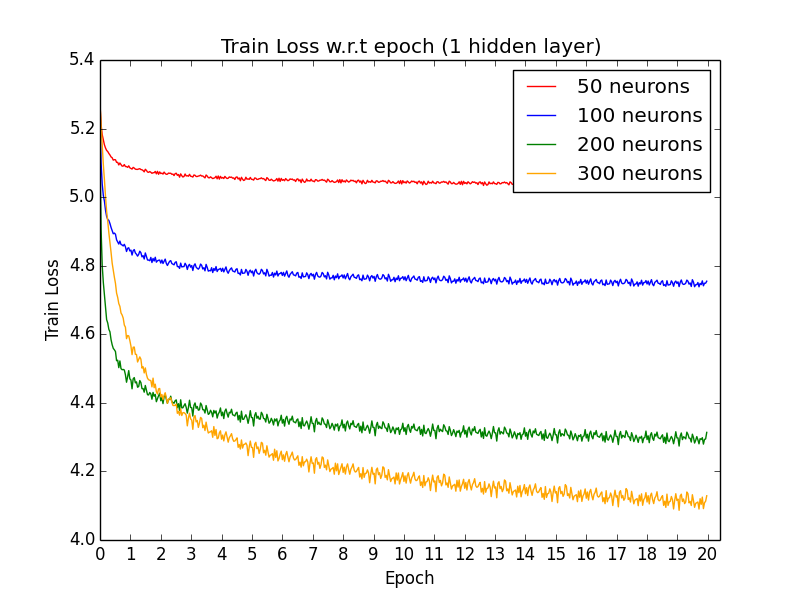
\includegraphics[scale=0.8]{train_1.png}
\end{center}

\vspace{7mm}

\begin{table}[H]
\label{T:equipos}
\begin{center}
\begin{tabular}{| c | c |}
\hline
\textbf{No. of Neurons in Hidden Layer} & \textbf{Validation accuracy($\%$) for 20 epochs} \\ 
\hline

50 & 75.92  \\ \hline
100 & 81 \\ \hline
200 & 81.02  \\ \hline
300 & 76.66  \\ \hline

\end{tabular}
\end{center}
\end{table}

\begin{center}
    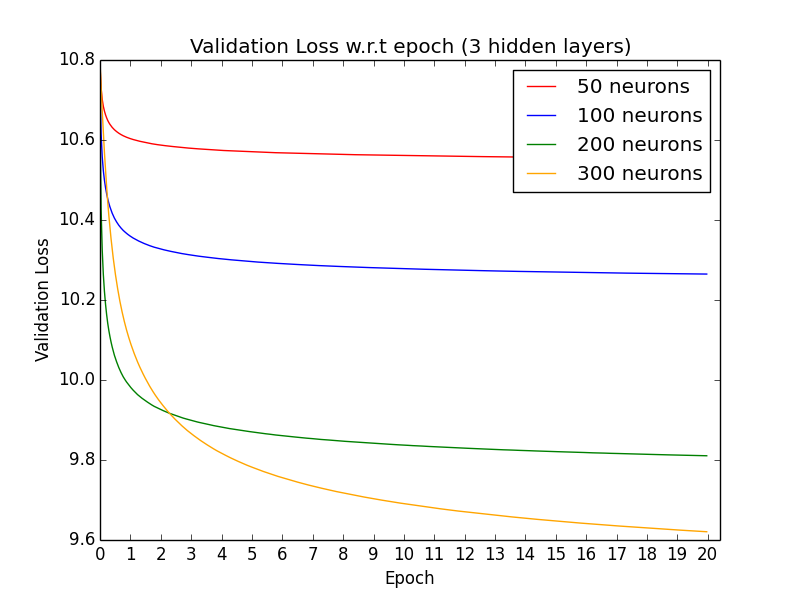
\includegraphics[scale=0.8]{val_1}
\end{center}

\subsection{No. of Hidden Layers : 2}
Hyperparameters used :
\begin{table}[H]
\label{T:equipos}
\begin{center}
\begin{tabular}{| c | c |}
\hline
\multicolumn{2}{| c |}{\textbf{Hyperparameters}} \\ 
\hline

Activation & Sigmoid  \\ \hline
Loss & Cross Entropy \\ \hline
Optimiser & Adam  \\ \hline
Batch size & 20  \\ \hline

\end{tabular}
\end{center}
\end{table}

\begin{center}
    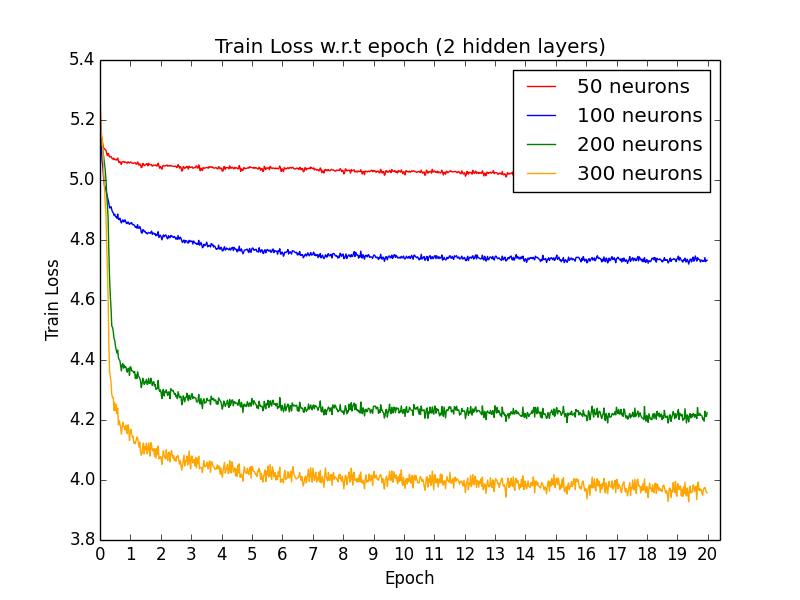
\includegraphics[scale=0.8]{train_2}
\end{center}

\vspace{7mm}

\begin{table}[H]
\label{T:equipos}
\begin{center}
\begin{tabular}{| c | c |}
\hline
\textbf{No. of Neurons in Hidden Layer} & \textbf{Validation accuracy($\%$) for 20 epochs} \\ 
\hline

50 & 79.9  \\ \hline
100 & 81.5 \\ \hline
200 & 85.26  \\ \hline
300 & 86.5  \\ \hline

\end{tabular}
\end{center}
\end{table}

\begin{center}
    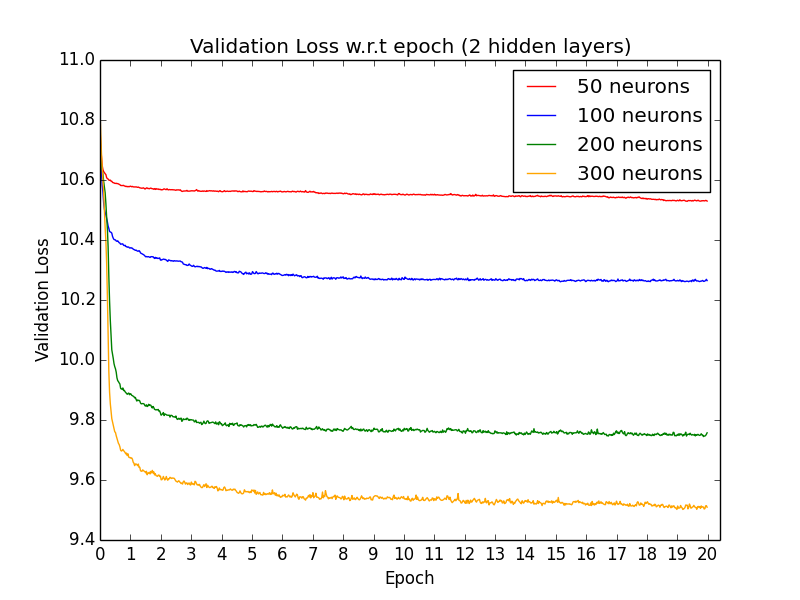
\includegraphics[scale=0.8]{val_2}
\end{center}

\subsection{No. of Hidden Layers : 3}
Hyperparameters used :
\begin{table}[H]
\label{T:equipos}
\begin{center}
\begin{tabular}{| c | c |}
\hline
\multicolumn{2}{| c |}{\textbf{Hyperparameters}} \\ 
\hline

Activation & Sigmoid  \\ \hline
Loss & Cross Entropy \\ \hline
Optimiser & Adam  \\ \hline
Batch size & 20  \\ \hline

\end{tabular}
\end{center}
\end{table}

\begin{center}
    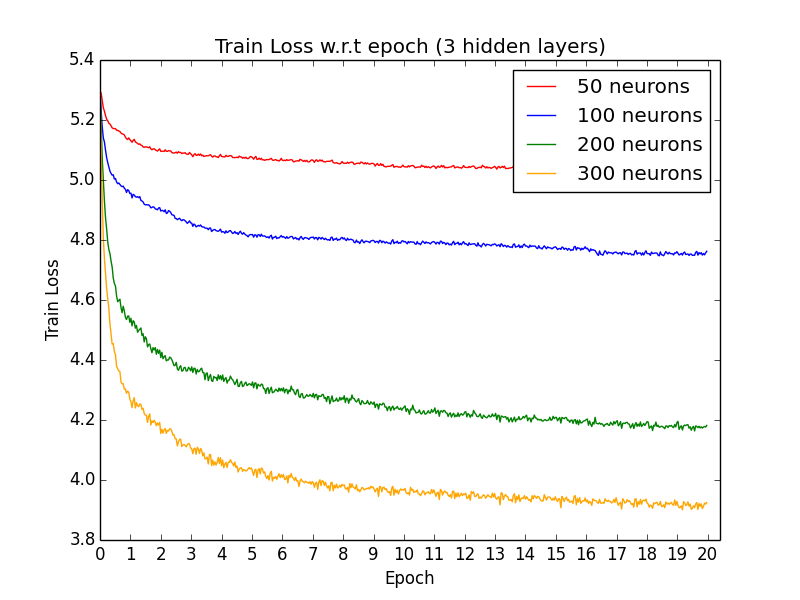
\includegraphics[scale=0.8]{train_3}
\end{center}

\vspace{7mm}

\begin{table}[H]
\label{T:equipos}
\begin{center}
\begin{tabular}{| c | c |}
\hline
\textbf{No. of Neurons in Hidden Layer} & \textbf{Validation accuracy($\%$) for 20 epochs} \\ 
\hline

50 & 86.54  \\ \hline
100 & 87.64 \\ \hline
200 & 88.26  \\ \hline
300 & 87.82  \\ \hline

\end{tabular}
\end{center}
\end{table}


\begin{center}
    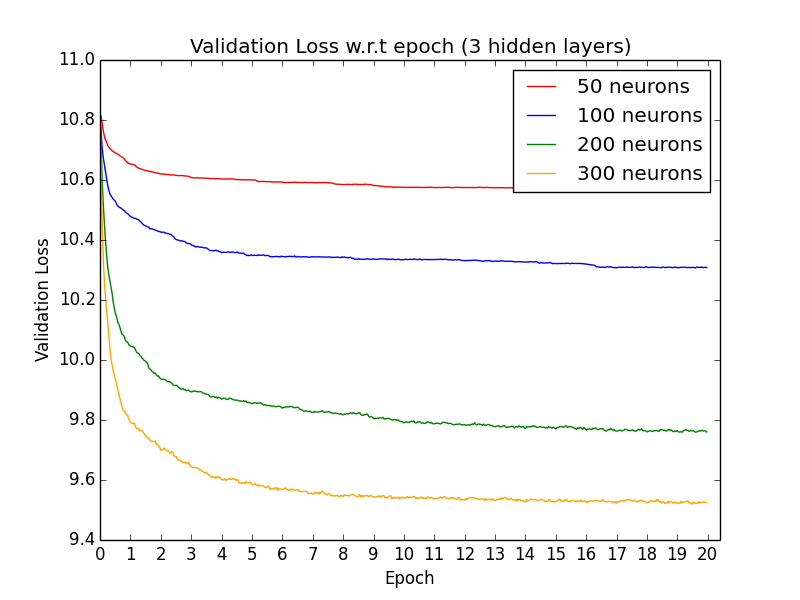
\includegraphics[scale=0.8]{val_3}
\end{center}

\subsection{No. of Hidden Layers : 4}
Hyperparameters used :
\begin{table}[H]
\label{T:equipos}
\begin{center}
\begin{tabular}{| c | c |}
\hline
\multicolumn{2}{| c |}{\textbf{Hyperparameters}} \\ 
\hline

Activation & Sigmoid  \\ \hline
Loss & Cross Entropy \\ \hline
Optimiser & Adam  \\ \hline
Batch size & 20  \\ \hline

\end{tabular}
\end{center}
\end{table}

\begin{center}
    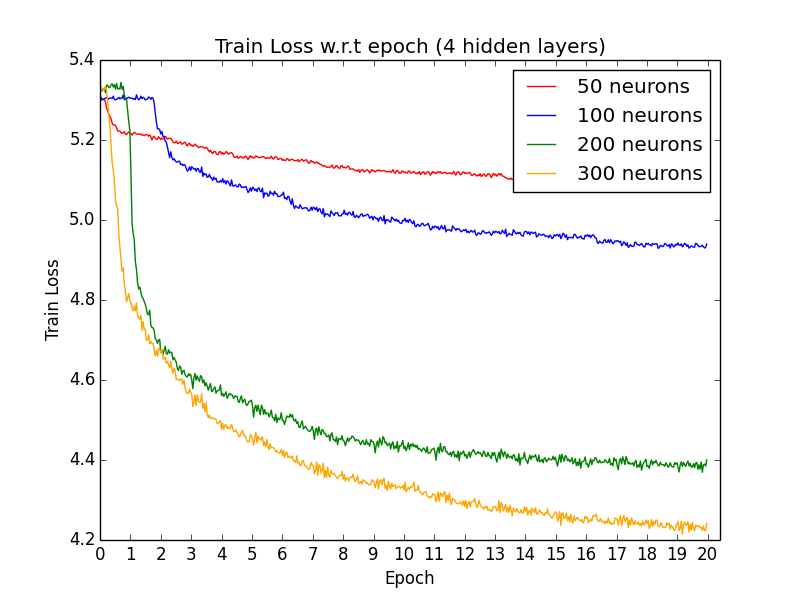
\includegraphics[scale=0.8]{train_4}
\end{center}


\vspace{7mm}

\begin{table}[H]
\label{T:equipos}
\begin{center}
\begin{tabular}{| c | c |}
\hline
\textbf{No. of Neurons in Hidden Layer} & \textbf{Validation accuracy($\%$) for 20 epochs} \\ 
\hline

50 & 64.6  \\ \hline
100 & 77.76 \\ \hline
200 & 87.62  \\ \hline
300 & 87.2  \\ \hline

\end{tabular}
\end{center}
\end{table}


\begin{center}
    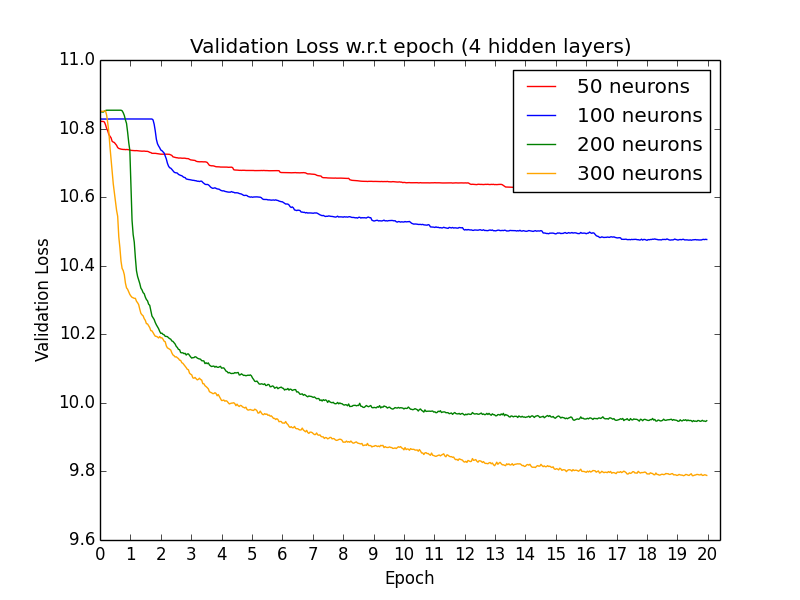
\includegraphics[scale=0.8]{val_4}
\end{center}

\subsection{Adam, NAG, Momentum, GD}
Hyperparameters used :
\begin{table}[H]
\label{T:equipos}
\begin{center}
\begin{tabular}{| c | c |}
\hline
\multicolumn{2}{| c |}{\textbf{Hyperparameters}} \\ 
\hline

Activation & Sigmoid  \\ \hline
Loss & Cross Entropy \\ \hline
No. of Hidden Layers & 3 (300,300,300)  \\ \hline
Batch size & 20  \\ \hline

\end{tabular}
\end{center}
\end{table}

\begin{center}
    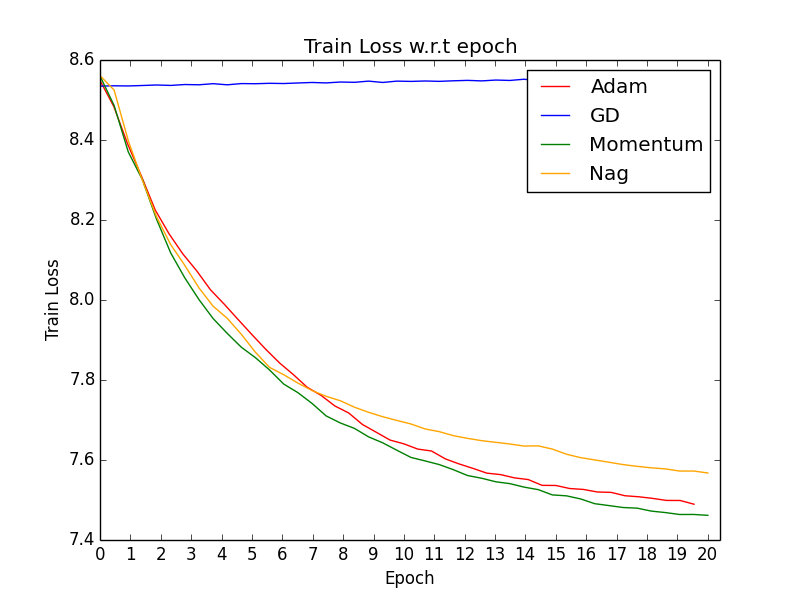
\includegraphics[scale=0.8]{train_5}
\end{center}

\begin{center}
    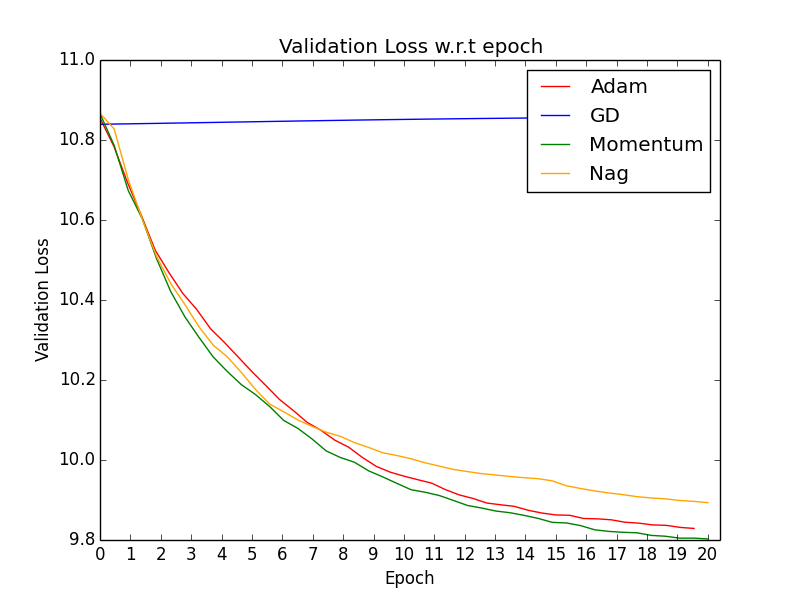
\includegraphics[scale=0.8]{val_5}
\end{center}


Adam : \\
%python train.py --lr 0.001 --momentum 0.75 --num_hidden 3 --sizes 300,300,300 --activation sigmoid --loss ce --opt gd --batch_size 500 --anneal true --save_dir pa1/ --expt_dir pa1/exp1/ --train train.csv --test test.csv
Nag : \\
%python train.py --lr 0.01 --momentum 0.75 --num_hidden 3 --sizes 300,300,300 --activation sigmoid --loss ce --opt gd --batch_size 500 --anneal true --save_dir pa1/ --expt_dir pa1/exp1/ --train train.csv --test test.csv



\subsection{sigmoid v/s tanh}
Hyperparameters used :
\begin{table}[H]
\label{T:equipos}
\begin{center}
\begin{tabular}{| c | c |}
\hline
\multicolumn{2}{| c |}{\textbf{Hyperparameters}} \\ 
\hline

Optimiser & Adam  \\ \hline
Loss & Cross Entropy \\ \hline
No. of Hidden Layers & 2 (100,100)  \\ \hline
Batch size & 20  \\ \hline

\end{tabular}
\end{center}
\end{table}

\begin{center}
    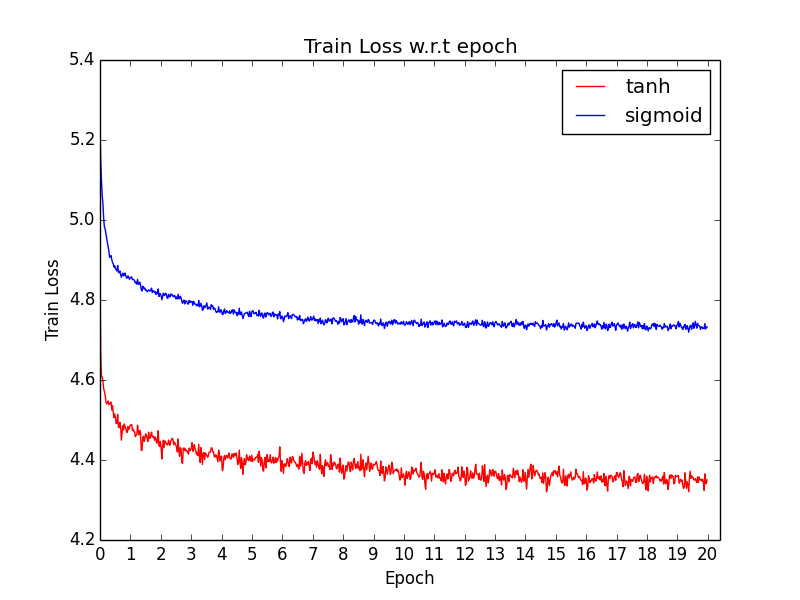
\includegraphics[scale=0.8]{train_6}
\end{center}

\begin{center}
    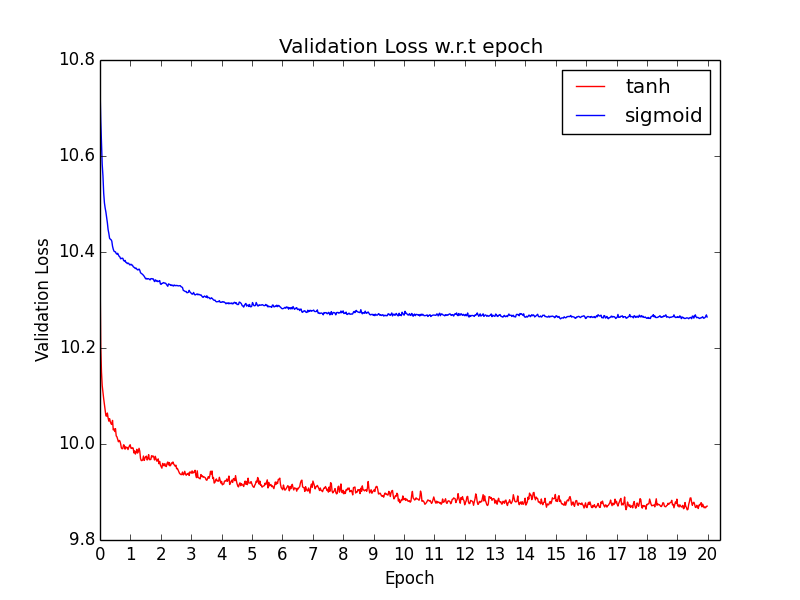
\includegraphics[scale=0.8]{val_6}
\end{center}

\subsection{cross entropy loss v/s squared error loss}
Hyperparameters used :
\begin{table}[H]
\label{T:equipos}
\begin{center}
\begin{tabular}{| c | c |}
\hline
\multicolumn{2}{| c |}{\textbf{Hyperparameters}} \\ 
\hline

Activation & Sigmoid  \\ \hline
Optimiser & Adam \\ \hline
No. of Hidden Layers & 2 (100,100)  \\ \hline
Batch size & 20  \\ \hline

\end{tabular}
\end{center}
\end{table}

\begin{center}
    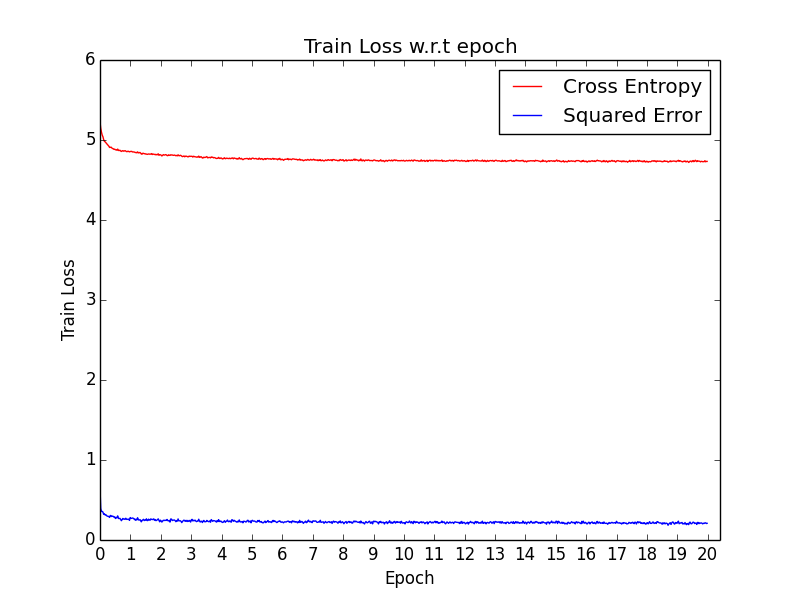
\includegraphics[scale=0.8]{train_7}
\end{center}

\begin{center}
    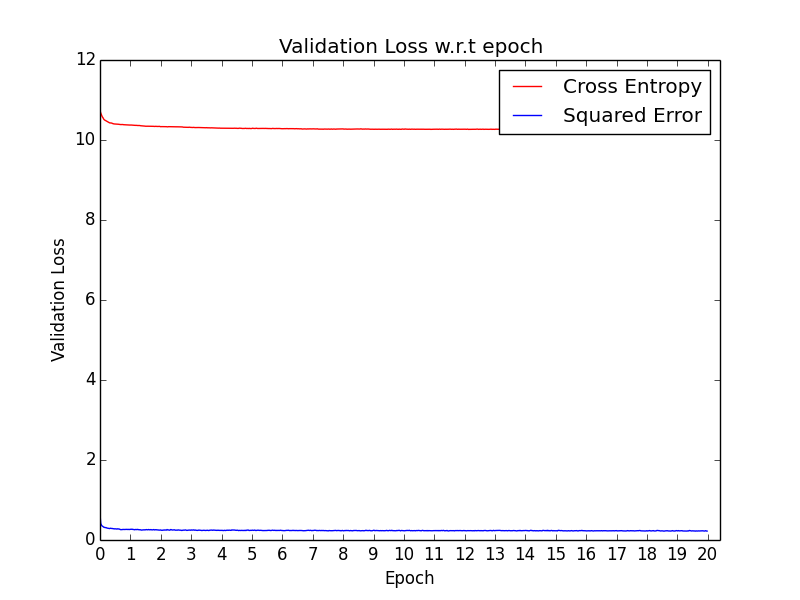
\includegraphics[scale=0.8]{val_7}
\end{center}

\section{Best Model}
Hyperparameters used :
\begin{table}[H]
\label{T:equipos}
\begin{center}
\begin{tabular}{| c | c |}
\hline
\multicolumn{2}{| c |}{\textbf{Hyperparameters}} \\ 
\hline

Activation & tanh  \\ \hline
Optimiser & Adam \\ \hline
No. of Hidden Layers & 3 (128,256,256)  \\ \hline
Batch size & 20  \\ \hline
Loss & Cross Entropy \\ \hline
Learning rate & 0.001 \\ \hline

\end{tabular}
\end{center}
\end{table}

Kaggle score = 88.766\\
Accuracy on validation = 88.6

\textbf{Other Submissions :}\\
\begin{enumerate}
    \item Submission filename : test$\_$submission.csv\\
    Hyperparameters used :
\begin{table}[H]
\label{T:equipos}
\begin{center}
\begin{tabular}{| c | c |}
\hline
\multicolumn{2}{| c |}{\textbf{Hyperparameters}} \\ 
\hline

Activation & tanh  \\ \hline
Optimiser & Adam \\ \hline
No. of Hidden Layers & 1 (300)  \\ \hline
Batch size & 20  \\ \hline
Loss & Cross Entropy \\ \hline
Learning rate & 0.001 \\ \hline

\end{tabular}
\end{center}
\end{table}

Kaggle score = 82.066\\
Accuracy on validation = 82
   
    \item Submission filename : test$\_$submission100.csv \\
    Hyperparameters used :
\begin{table}[H]
\label{T:equipos}
\begin{center}
\begin{tabular}{| c | c |}
\hline
\multicolumn{2}{| c |}{\textbf{Hyperparameters}} \\ 
\hline

Activation & tanh  \\ \hline
Optimiser & Adam \\ \hline
No. of Hidden Layers & 3 (100,100,100)  \\ \hline
Batch size & 20  \\ \hline
Loss & Cross Entropy \\ \hline
Learning rate & 0.001 \\ \hline

\end{tabular}
\end{center}
\end{table}

Kaggle score = 87.06\\
Accuracy on validation = 88.26

    \item Submission filename : test$\_$submission300.csv \\
    Hyperparameters used :
\begin{table}[H]
\label{T:equipos}
\begin{center}
\begin{tabular}{| c | c |}
\hline
\multicolumn{2}{| c |}{\textbf{Hyperparameters}} \\ 
\hline

Activation & tanh  \\ \hline
Optimiser & Adam \\ \hline
No. of Hidden Layers & 3 (300,300,300)  \\ \hline
Batch size & 20  \\ \hline
Loss & Cross Entropy \\ \hline
Learning rate & 0.001 \\ \hline

\end{tabular}
\end{center}
\end{table}

Kaggle score = 88.4\\
Accuracy on validation = 88.26

\item Submission filename : test$\_$submission300.csv \\
Hyperparameters used :
\begin{table}[H]
\label{T:equipos}
\begin{center}
\begin{tabular}{| c | c |}
\hline
\multicolumn{2}{| c |}{\textbf{Hyperparameters}} \\ 
\hline

Activation & tanh  \\ \hline
Optimiser & Adam \\ \hline
No. of Hidden Layers & 3 (300,300,300)  \\ \hline
Batch size & 20  \\ \hline
Loss & Cross Entropy \\ \hline
Learning rate & 0.001 \\ \hline

\end{tabular}
\end{center}
\end{table}

Kaggle score = 88.4\\
Accuracy on validation = 88.26


\item Submission filename: sub$\_$2.csv\\
Hyperparameters used :
\begin{table}[H]
\label{T:equipos}
\begin{center}
\begin{tabular}{| c | c |}
\hline
\multicolumn{2}{| c |}{\textbf{Hyperparameters}} \\ 
\hline

Activation & sigmoid  \\ \hline
Optimiser & Adam \\ \hline
No. of Hidden Layers & 3 (300,300)  \\ \hline
Batch size & 20  \\ \hline
Loss & Cross Entropy \\ \hline
Learning rate & 0.001 \\ \hline

\end{tabular}
\end{center}
\end{table}

Kaggle score = 86.5\\


\item Submission filename: sub3.csv
Hyperparameters used :
\begin{table}[H]
\label{T:equipos}
\begin{center}
\begin{tabular}{| c | c |}
\hline
\multicolumn{2}{| c |}{\textbf{Hyperparameters}} \\ 
\hline

Activation & sigmoid  \\ \hline
Optimiser & Adam \\ \hline
No. of Hidden Layers & 2 (200,200)  \\ \hline
Batch size & 200  \\ \hline
Loss & Cross Entropy \\ \hline
Learning rate & 0.005 \\ \hline

\end{tabular}
\end{center}
\end{table}

Kaggle score = 88.4\\



\end{enumerate}

 \textbf{NOTE : }\\
 \begin{itemize}
     \item Even though the best \textbf{kaggle} submission was observed for the above set of hyperparameters, we got to know we had to pickle the model later on and hence due to the unavailability of resources and time(as other codes were running during the time), the weights submitted are for a sub-optimal model which gives an accuracy around 0.5$\%$ less than our best submission.
     \item \textbf{sklearn} has been used only for calculating accuracy and for no other purpose
 \end{itemize}

%-------------------------------------------------------------------------------
% REFERENCES
%-------------------------------------------------------------------------------
\begin{thebibliography}{9}
\bibitem{1} 
Mitesh M Khapra. \textit{CS7015 Deep Learning: Lecture 5}, 
Indian Institute of Technology Madras, 2018
\end{thebibliography}


\end{document}

%-------------------------------------------------------------------------------
% SNIPPETS
%-------------------------------------------------------------------------------

%\begin{figure}[!ht]
%	\centering
%	\includegraphics[width=0.8\textwidth]{file_name}
%	\caption{}
%	\centering
%	\label{label:file_name}
%\end{figure}

%\begin{figure}[!ht]
%	\centering
%	\includegraphics[width=0.8\textwidth]{graph}
%	\caption{Blood pressure ranges and associated level of hypertension (American Heart Association, 2013).}
%	\centering
%	\label{label:graph}
%\end{figure}

%\begin{wrapfigure}{r}{0.30\textwidth}
%	\vspace{-40pt}
%	\begin{center}
%		\includegraphics[width=0.29\textwidth]{file_name}
%	\end{center}
%	\vspace{-20pt}
%	\caption{}
%	\label{label:file_name}
%\end{wrapfigure}

%\begin{wrapfigure}{r}{0.45\textwidth}
%	\begin{center}
%		\includegraphics[width=0.29\textwidth]{manometer}
%	\end{center}
%	\caption{Aneroid sphygmomanometer with stethoscope (Medicalexpo, 2012).}
%	\label{label:manometer}
%\end{wrapfigure}

%\begin{table}[!ht]\footnotesize
%	\centering
%	\begin{tabular}{cccccc}
%	\toprule
%	\multicolumn{2}{c} {Pearson's correlation test} & \multicolumn{4}{c} {Independent t-test} \\
%	\midrule	
%	\multicolumn{2}{c} {Gender} & \multicolumn{2}{c} {Activity level} & \multicolumn{2}{c} {Gender} \\
%	\midrule
%	Males & Females & 1st level & 6th level & Males & Females \\
%	\midrule
%	\multicolumn{2}{c} {BMI vs. SP} & \multicolumn{2}{c} {Systolic pressure} & \multicolumn{2}{c} {Systolic Pressure} \\
%	\multicolumn{2}{c} {BMI vs. DP} & \multicolumn{2}{c} {Diastolic pressure} & \multicolumn{2}{c} {Diastolic pressure} \\
%	\multicolumn{2}{c} {BMI vs. MAP} & \multicolumn{2}{c} {MAP} & \multicolumn{2}{c} {MAP} \\
%	\multicolumn{2}{c} {W:H ratio vs. SP} & \multicolumn{2}{c} {BMI} & \multicolumn{2}{c} {BMI} \\
%	\multicolumn{2}{c} {W:H ratio vs. DP} & \multicolumn{2}{c} {W:H ratio} & \multicolumn{2}{c} {W:H ratio} \\
%	\multicolumn{2}{c} {W:H ratio vs. MAP} & \multicolumn{2}{c} {\% Body fat} & \multicolumn{2}{c} {\% Body fat} \\
%	\multicolumn{2}{c} {} & \multicolumn{2}{c} {Height} & \multicolumn{2}{c} {Height} \\
%	\multicolumn{2}{c} {} & \multicolumn{2}{c} {Weight} & \multicolumn{2}{c} {Weight} \\
%	\multicolumn{2}{c} {} & \multicolumn{2}{c} {Heart rate} & \multicolumn{2}{c} {Heart rate} \\
%	\bottomrule
%	\end{tabular}
%	\caption{Parameters that were analysed and related statistical test performed for current study. BMI - body mass index; SP - systolic pressure; DP - diastolic pressure; MAP - mean arterial pressure; W:H ratio - waist to hip ratio.}
%	\label{label:tests}
%\end{table}